%\linenumbers*
\chapter{EFFECT OF TEMPORAL SCALES OF STORM DATA ON EROSION}
\label{sec:EFFECTSOFTEMPORALSCALESOFSTROMDATA}

\section{Introduction}
\label{sec:TemporalScalesEffectsIntroduction}

%******start with little bit of rationalization of this set of experiments and
%why did I choose to do THIS and why IN THIS WAY
When modelling soil erosion, finding suitable input data for the simulation is
an important but also difficult part of model-based researches. Ideally, input
data need to be measured directly from a study site and parametrized for a model
simulation. However, this process requires a great effort and time. It is also
frequently affected by geographical and financial situations of research. All
these reasons affect how rainfall data are made available in different scales
either spatially, temporally or both. Thus, we often end up using what is
readily available rather than what is originally required by erosion models.

Rainfall intensity is highly variable depending on data scales and where they
are measured from \citep{nyssen2005-172}. Consequently, using rainfall data
that have a undesired data scale for erosion simulations may produce unknown
implications that may later lead to inaccurate model outputs. Therefore, this
chapter aims to investigate effects of different temporal scales of rainfall
data on erosion model simulation processes. In addition, which data format
between CLIGEN and breakpoint data is more suitable for current research was
looked at.

The results of this chapter and the subsequent chapters attempts to provide some
answers for Research Question \ref{researchquestion2}:\
\begin{quotation}
Assuming that we use a model to predict erosion rates under the future climate
which may have different rainfall intensities from the present, what information
do we need to make predictions in terms of both climate and process
understanding?                                                      
\end{quotation}

\section{Simulation Data and Methods}
\label{sec:TemporalScalesEffectsMethods}
%******Need a section discussing what is meant by a ``storm'' and giving your
%own definition. You can then refer to this in the Conclusions.

There are two ways of defining average rainfall intensity. One is to calculate
kinetic energy of rainfall by measuring size, distribution and velocity of
raindrops. The other is to calculate it by dividing total rainfall amount by
rainfall duration. The latter is used in this research because erosion models
used here employ the latter concept when rainfall data are feed into the model
as inputs. Rainfall intensity is expressed as rainfall amount divided by time
(e.g.\ mm/hr) in this research.

The variations between data points such as breakpoints is termed as WSIV
(Within-Storm Intensity Variation) for convenience. This is related to temporal
scales of rainfall data as well as types of storms (convective and frontal). In
this research, unless specified, a rainfall storm or rainfall event is defined
as a daily rainfall. Consequences of this assumption were not covered in this
study simply because all models used here assume that a rainfall storm does not
last longer than a day. Nevertheless, this research recognises the presence
of this issue and the need for further studies on the definition of rainfall
storm.

%The most intense activity started at around 1900 GMT on 11 October 2000 and
%continued until 1000 GMT on 12 October 2000 \citep{saunders2001-360}. The
%return period for such a fall is estimated at around 300 years
%\citep{saunders2001-360}.
Two storms that occurred on 4 July 2000 and on 11 October 2000 for summer and
autumn, respectively, were selected from Plumpton event rainfall data (Table
\ref{tab:DetailsOfDataStations}). 
The tipping-bucket data for both events were aggregated into 5 different
temporal scales---1, 5, 15, 30 and 60 minutes. This was done to simulate
different temporal scaled rainfall data. Each temporal scale was treated as if
it was the ``original'' scale for the data with these being the only records
available. Two sets of temporally varying summer and autumn storm data were
prepared into CLIGEN data format and breakpoint data format for erosion
estimations.

CLIGEN rainfall data describe rainfall characteristics with four parameters:
total rainfall amount ($R$, inch), effective rainfall duration ($D$, minute),
normalised time to peak ($t_p$) and normalised peak intensity ($i_p$). Effective
daily rainfall duration was calculated by summing the number of temporal bins
with rainfall on the event day, after removing temporal bins without rainfall.
Effects of removing these ``gaps'' are investigated in the following section,
Chapter \ref{sec:EFFECTSOFCONTINOUSANDDISCONTINUSSTORM}. Normalised time to
peak is a relative time of peak intensity after the removal of gaps.
Normalised peak intensity is a peak intensity that is relative to average
rainfall intensity of the storm. These four parameters were calculated
individually for each time-stepped data (Table
\ref{tab:CLIGENWEPPInputFileParameters}), and weather inputs for WEPP were
built (Appendix \ref{sec:WEPPInputData}). Breakpoint data, on the other hand,
consist of two parameters: rainfall (accumulated) time and rainfall
(accumulated) amounts or intensity. Each dataset was converted into these two
parameters, and the number of breakpoints is counted.

Two process-based erosion models, WEPP and EUROSEM, were used at the current
stage to simulate runoff and soil loss. WEPP originally requires CLIGEN rainfall
data which are stochastically generated using the statistical properties of
15-min rainfall data. CLIGEN data and breakpoint data prepared from rainfall
data with 1, 5, 15, 30 and 60-min temporal scale were used to look at the effect
of different temporal scale. EUROSEM was also used since it has been
designed to use breakpoint rainfall data. Therefore, it would be a good
comparison to WEPP which has been originally designed to use CLIGEN data
although breakpoint data could also be used.
%why was RillGrow not used??

As mentioned, EUROSEM uses breakpoint rainfall data only. Thus, unless the
EUROSEM code was rewritten, using CLIGEN data directly with EUROSEM is not
possible. To use CLIGEN data for EUROSEM simulations, an additional
procedure was carried out to make sure that the same rainfall data were used
as for WEPP simulations. According to WEPP model document, WEPP disaggregates
CLIGEN data into 10 breakpoints using a double exponential equation before
calculating erosion related parameters \citep{flanagan1995-usda}. The
disaggregated rainfall data can be found in the WEPP output files. For EUROSEM
simulations, CLIGEN data were used as these ``WEPP-disaggregated'' rainfall
data which is in the form of breakpoint data.
%Issues that might arise using this approach are discussed in the later section
%(Section \ref{sec:tpipbpDiscussion}).

Other inputs for EUROSEM were adopted from WEPP outputs as no direct
measurements were available to build EUROSEM inputs from scratch. This approach
may be problematic for certain modelling studies. However, in this research, it
permits a workaround to problems of unavailable factors for EUROSEM simulation.
It needs to be noted that the emphasis of this research is not on assessing the
performance of models against measured data.

The effect of the temporal scales on rainfall intensity and on runoff and soil
loss were examined. For comparison purpose, 15-min data were used as a reference
scale when comparisons were done to highlight the effects. Also, this scale is
the scale that were used for the CLIGEN development.

%WEPP-disaggregated rainfall data were obtained from the WEPP outputs and
%used as EUROSEM rainfall inputs. This is because EUROSEM only uses
%breakpoint data rather than CLIGEN-generated rainfall data. When
%CLIGEN-generated rainfall data are fed into WEPP, WEPP disaggregates the
%rainfall data into rainfall intensity patterns using a double exponential
%function . These disaggregated rainfall data are similar to breakpoint
%data. The procedure on how WEPP disaggregates rainfall is described in
%\citet{flanagan1995-usda}.

%For both storms, only amount ($R$), duration ($D$), normalised time to peak
%intensity ($t_p$) and normalised peak intensity $i_p$ were adjusted
%accordingly. All other parameters, far from these four parameters, in the
%weather input were kept unchanged for the simulations.

%%It may be a good idea to compare, or at least, talk  about little bit about
%%the effects caused by using CLIGEN data or breakpoint data. By using one or
%%another, are the effects enhanced or subdued for individual time scales,
%%and also for overall?

%Temporal scale variation results with BP, TP \& IP
% EUROSEM simulation results
% WEPP simulation results
%   - WEPP interpreted rainfall intensity information

\section{Effects on Rainfall Intensity Information}
\label{sec:EffectsOnRainfallIntensityInput}
The highest rainfall amount in Plumpton was 133.8 mm recorded on 11 October
2000. This  event at Plumpton on 11 October 2000 was considered responsible for
the recent severe soil erosion and flooding in the area \citep{boardman2001-346,
marsh2001-343, saunders2001-360}. The duration of this event was 1208 minutes
(i.e.\ 20 hours and 8 minutes). Average intensity for this rainfall was 6.65
mm/hr. 1-min peak intensity was 84 mm/hr. Typical summer rainfall was recorded
on 4 July 2000. Total rainfall amount was 74.8 mm and durations was 808 minutes
(about 13.5 hours). Average intensity for this event was 5.5 mm/hr while 1-min
peak intensity reached 60 mm/hr. The details of two events are summarised in
Table \ref{tab:DetailsoftworainstormsobservedinPlumpton}.

\begin{table}[htbp]
  \figureversion{tabular}
  \centering
  \small
  \caption{Details of two rain storms observed in Plumpton}
  \label{tab:DetailsoftworainstormsobservedinPlumpton}
    \begin{tabular}{lcc}
    \toprule
     & 11 October 2000 & 4 July 2000 \\
    \midrule
    Amount (mm) & 133.8 & 74.8\\
    Total duration (min) & 1208 & 808 \\
    Average intensity (mm/hr) & 6.7 & 5.5 \\
    Effective duration (min) & 460 & 313 \\
    1-min peak intensity (mm/hr) & 84 & 60 \\
    \bottomrule
    \end{tabular}
\end{table}

WEPP weather input data for two storms were built by obtaining rainfall amount,
duration, peak intensity and time to peak. These values are individually
calculated for each temporal scaled data. The details of the input parameters
are shown in Table \ref{tab:CLIGENWEPPInputFileParameters}.

\begin{table}[htbp]
  \figureversion{tabular}
  \centering
  \small
  \caption{CLIGEN data parameters for two rain storms observed in
Plumpton}
  \label{tab:CLIGENWEPPInputFileParameters}
    \begin{tabular}{rcccccccc} \toprule
       & \multicolumn{4}{c}{11 October 2000} &
\multicolumn{4}{c}{4 July 2000}\\
       \cmidrule(r){2-5} \cmidrule(l){6-9}
       & amount & duration$^{\dagger}$ & $t_p$ & $i_p$ & amount &
duration$^{\dagger}$ & $t_p$ & $i_p$\\
       %\addlinespace[-1mm]
       & \scriptsize(mm) & \scriptsize(hr) & & & \scriptsize(mm) &
\scriptsize(hr) & & \\
       \midrule
      1-min  & 133.8 & 7.4  & 0.12 & 4.64 & 74.8 & 5.2  & 0.63 & 4.20\\
      5-min  & 133.8 & 12.8 & 0.46 & 5.53 & 74.8 & 11.1 & 0.58 & 6.41\\
      15-min & 133.8 & 15.5 & 0.49 & 2.87 & 74.8 & 13.3 & 0.54 & 3.69\\
      30-min & 133.8 & 17   & 0.93 & 2.69 & 74.8 & 14   & 0.52 & 2.95\\
      60-min & 133.8 & 18   & 0.64 & 2.23 & 74.8 & 14   & 0.54 & 2.65\\
      \bottomrule
      %\addlinespace[1mm]
      \multicolumn{9}{l}{\footnotesize $^\dagger$ Effective rainfall
duration, {\normalsize{$t_p$}}: Normalised time-to-peak, {\normalsize{$i_p$}}:
Normalised peak intensity}
    \end{tabular}
\end{table}

For CLIGEN data (Table \ref{tab:CLIGENWEPPInputFileParameters}), each set of
temporally varying rainfall data shows different total rainfall durations
depending on what time interval they were aggregated into. Effective rainfall
duration increases as the data scale increases. Peak rainfall intensities are
also affected by the data scale while total rainfall amounts are the same. This
means that only rainfall intensity information is different for each temporal
scale. It is also found that the change of temporal scale can shift the temporal
location of peak intensity ($t_p$). This may change the shape of storms from,
for example, ascending intensity to descending intensity. Changes of the storm
shape are further investigated in Chapter
\ref{sec:EFFECTSOFRAINFALLINTENSITYCHANGESONSOILEROSION}.

For breakpoint data, the maximum numbers of time intervals per day are 1440,
288, 96, 48 and 24 for 1, 5, 15, 30 and 60-min data, respectively. The rainfall
data with different temporal scales show different rainfall intensity
information (Figure \ref{fig:dr_storm} and \ref{fig:pl_storm}). Higher temporal
resolution data show higher instantaneous peak rainfall intensities. With 1-min
data, for example, a peak rainfall intensity was over 80 mm/hr (Figure
\ref{fig:pl_storm-a}). In comparison, 60-min data show no peak rainfall
intensity higher than 20 mm/hr (Figure \ref{fig:pl_storm-e}). This is because
rainfall intensity is averaged over the length of each time step. Time to peak
rainfall intensity is also different for each temporal scale (Figure
\ref{fig:dr_storm} and \ref{fig:pl_storm}).

\begin{figure}[htbp]
  \centering
  % These are called DR storm but in fact they are Plumpton July storm
    \subfloat[]{\label{fig:dr_storm-a}
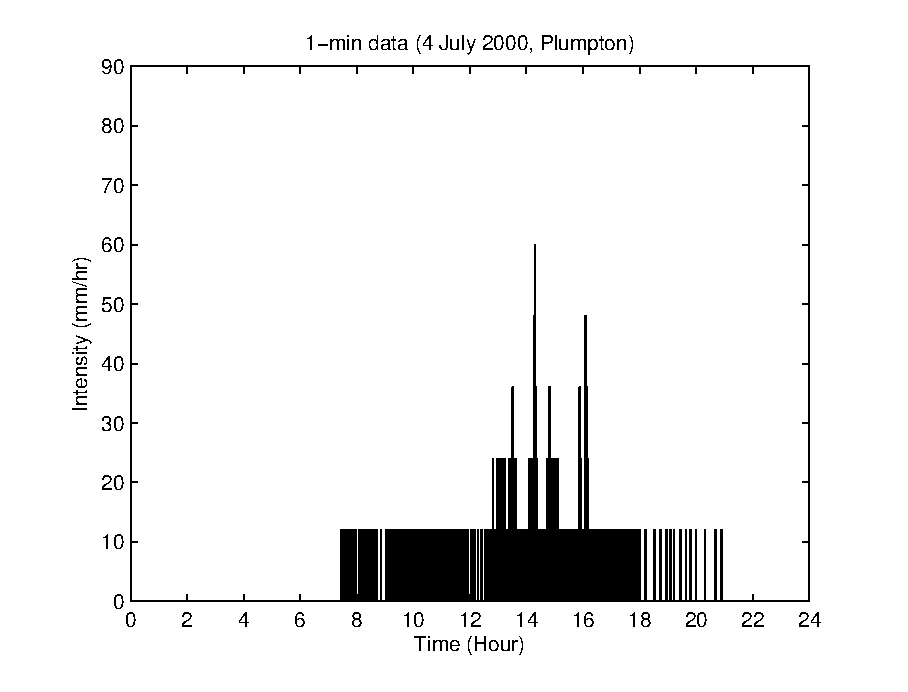
\includegraphics[width=0.49\textwidth]{./img/dr_storm_1min}}
    \subfloat[]{\label{fig:dr_storm-b}
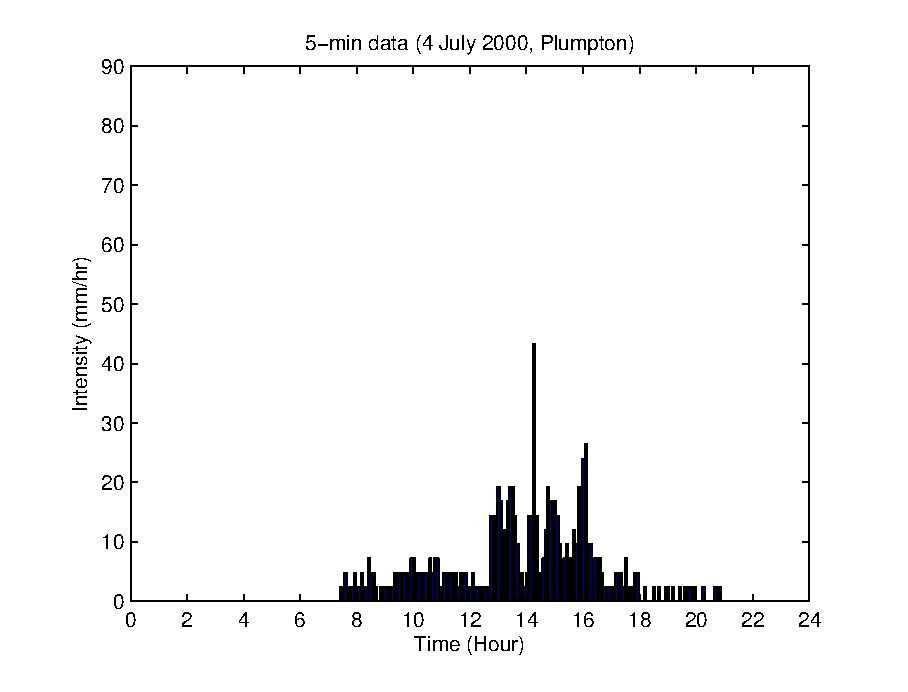
\includegraphics[width=0.49\textwidth]{./img/dr_storm_5min}}
    \qquad
    \subfloat[]{\label{fig:dr_storm-c}
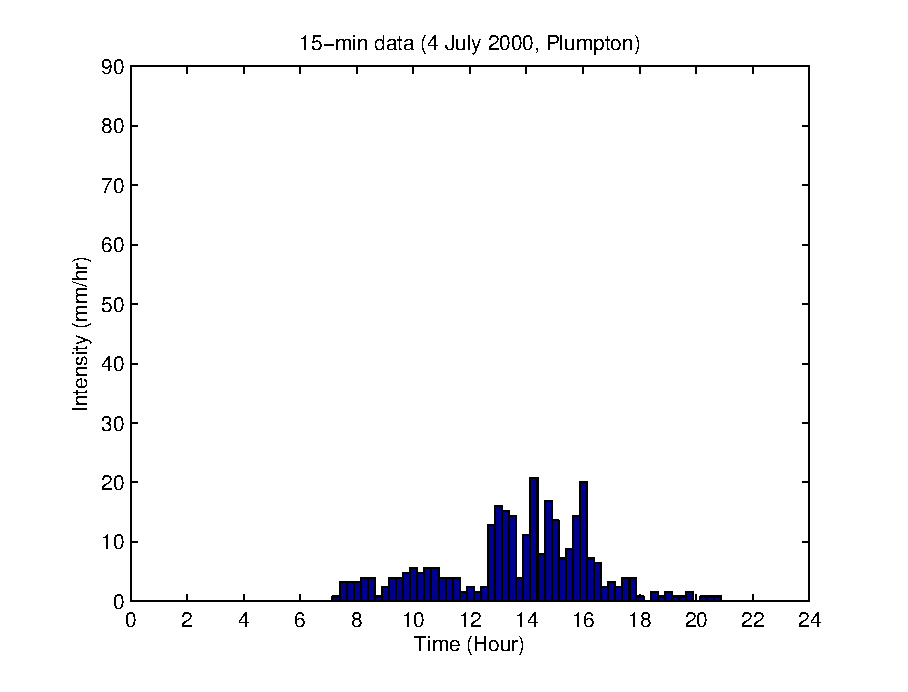
\includegraphics[width=0.5\textwidth]{./img/dr_storm_15min}}
    \qquad
    \subfloat[]{\label{fig:dr_storm-d}
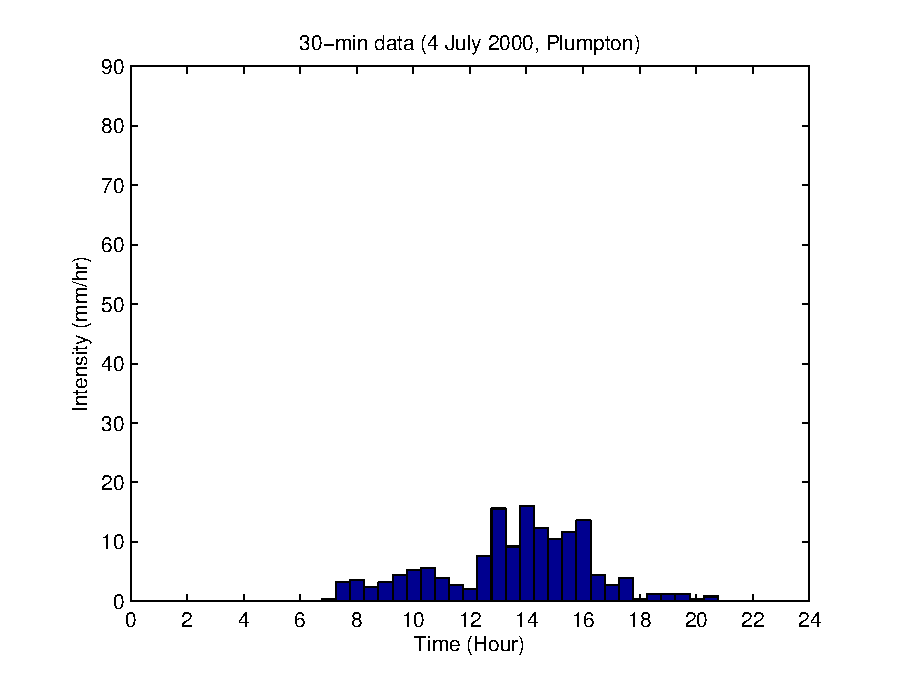
\includegraphics[width=0.49\textwidth]{./img/dr_storm_30min}}
    \subfloat[]{\label{fig:dr_storm-e}
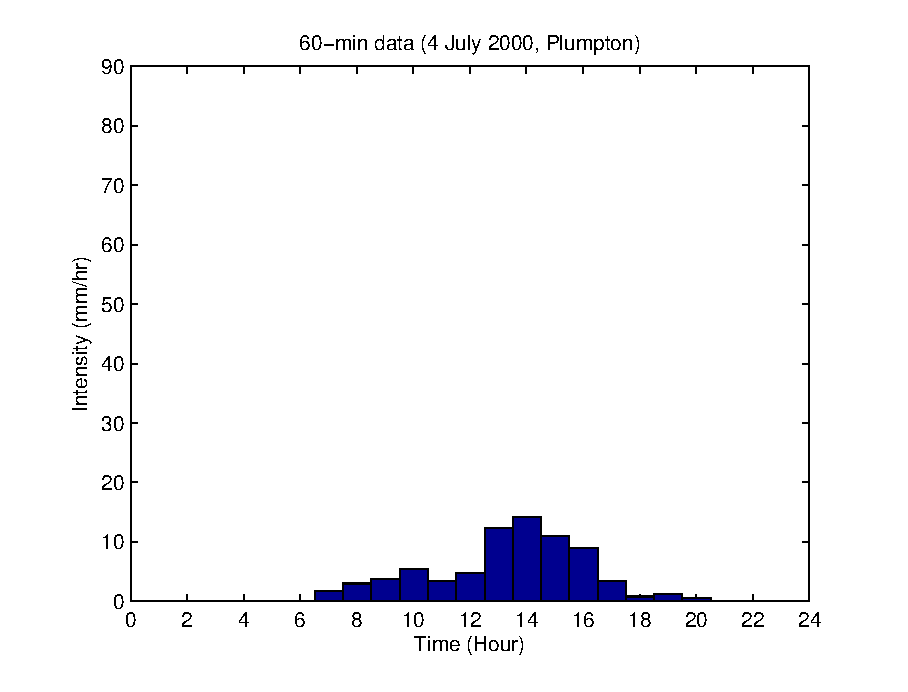
\includegraphics[width=0.49\textwidth]{./img/dr_storm_60min}}
  \caption{Various temporal scales of original breakpoint data for 4 July 2000
storm in Plumpton}
  \label{fig:dr_storm}
\end{figure}

\begin{figure}[htbp]
  \centering
    \subfloat[]{\label{fig:pl_storm-a}
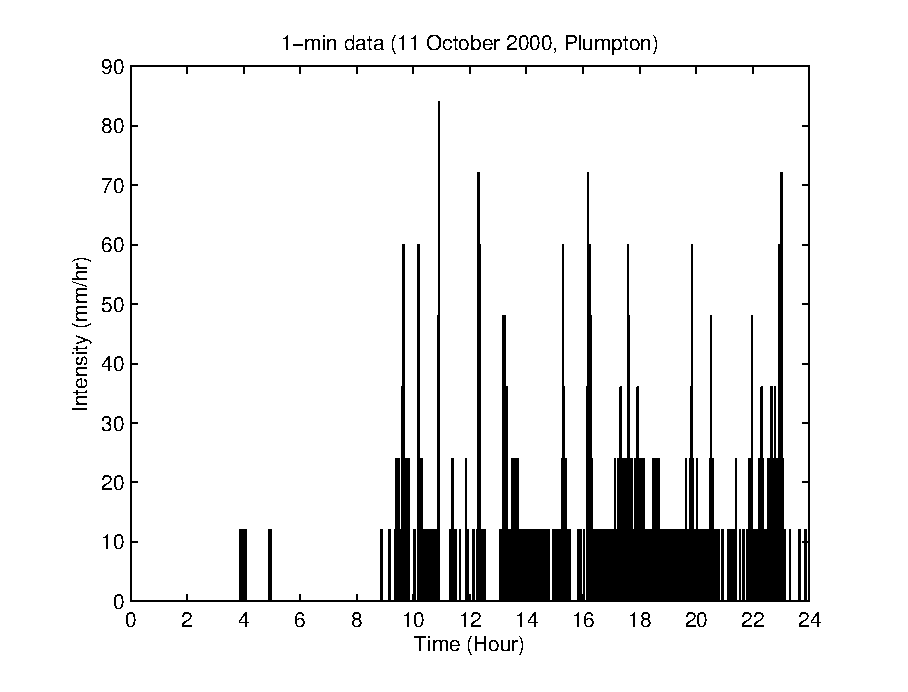
\includegraphics[width=0.49\textwidth]{./img/pl_storm_1min}}
    \subfloat[]{\label{fig:pl_storm-b}
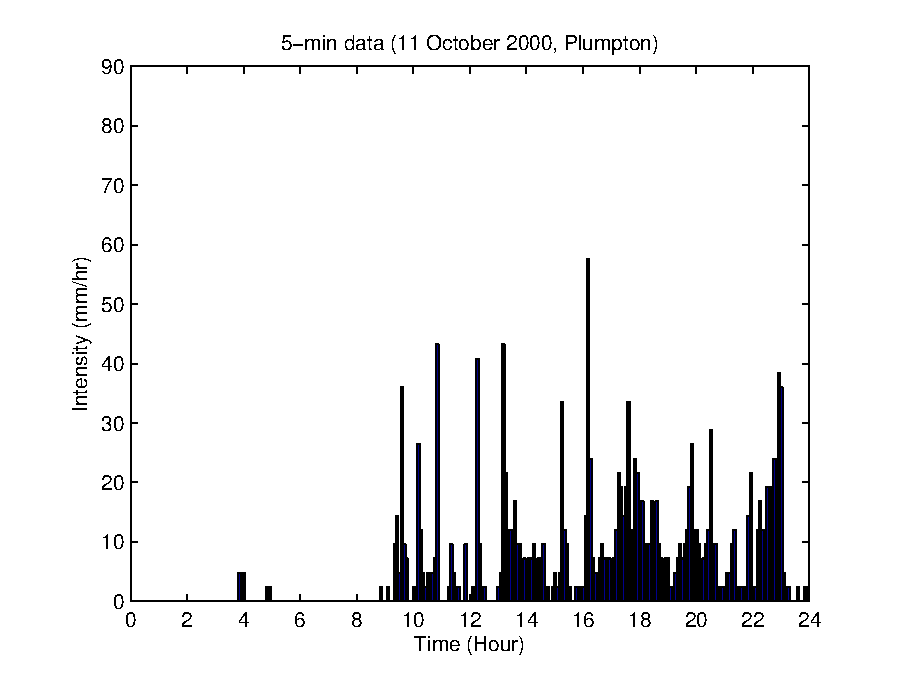
\includegraphics[width=0.49\textwidth]{./img/pl_storm_5min}}
    \qquad
    \subfloat[]{\label{fig:pl_storm-c}
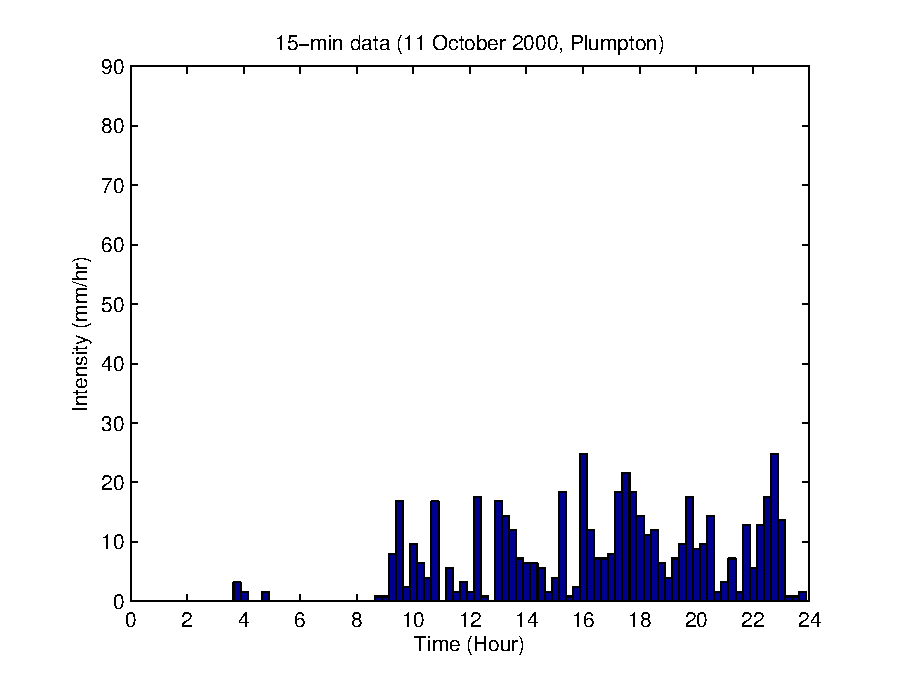
\includegraphics[width=0.5\textwidth]{./img/pl_storm_15min}}
    \qquad
    \subfloat[]{\label{fig:pl_storm-d}
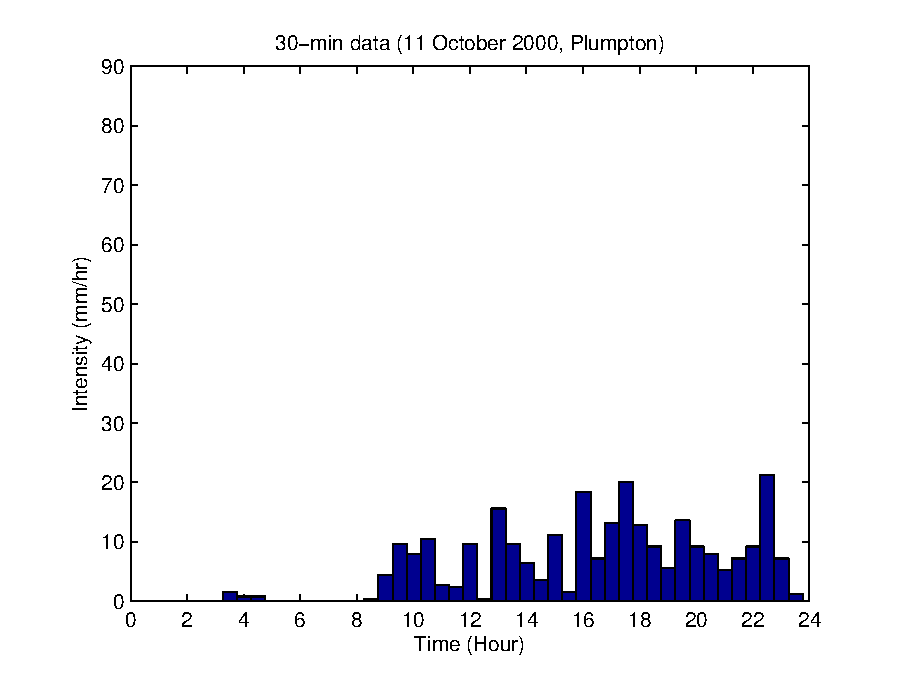
\includegraphics[width=0.49\textwidth]{./img/pl_storm_30min}}
    \subfloat[]{\label{fig:pl_storm-e}
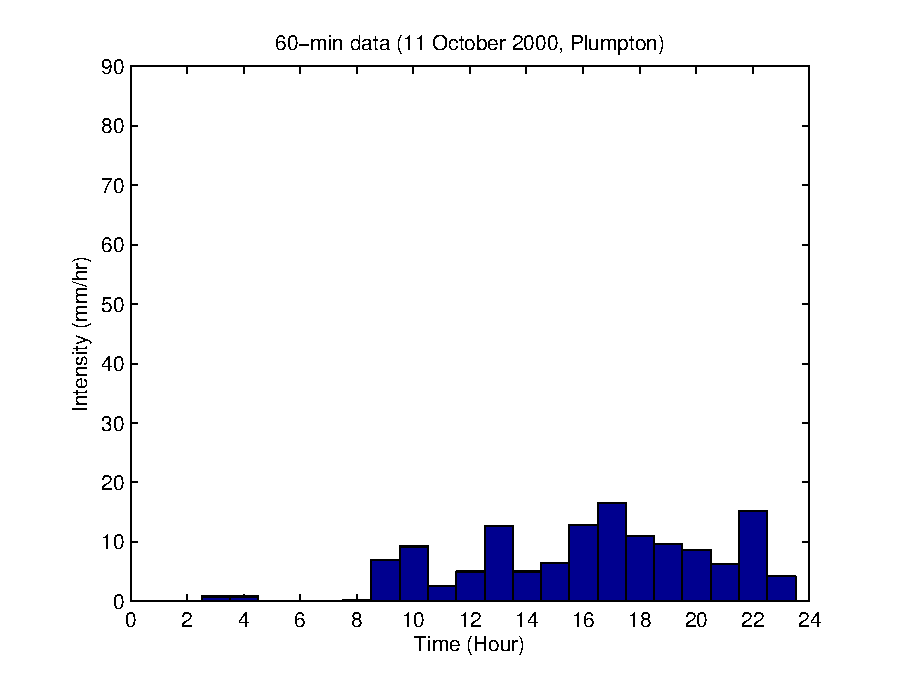
\includegraphics[width=0.49\textwidth]{./img/pl_storm_60min}}
  \caption{Various temporal scales of original breakpoint data for 11 October
2000 storm in Plumpton}
  \label{fig:pl_storm}
\end{figure}

\section{Effects on Simulated Runoff and Soil Loss}
\label{sec:TemporalScalesSimulatedRunoffAndSoilLoss}

The breakpoint data prepared for both October and July events with 1 and 5-min
time intervals could not be used for both erosion models because of model
limitations. It was found that WEPP and EUROSEM have a limit in the number of
breakpoints that they can process. Thus, no runoff and soil loss rates were
estimated with 1 and 5-min breakpoint data.

\subsection{Runoff}
\label{sec:TemporalScalesSimulatedRunoff}

In overall, both erosion models estimated greater runoff when rainfall data
with high temporal scales were used than when low temporal scaled data were
used. However, this is only true for CLIGEN data type. For breakpoint data
format, the effect of temporal data scales is rather unclear for both models.
% You need to be more specific about what you are trying to say here.

Runoff amounts estimated by WEPP for rainfall data with different time scales
are shown in Table
\ref{tab:DifferentTemporalScalesOfRainfallDataOnWEPPRunoffEstimation} and Figure
\ref{fig:wepp_roff_sloss_temp_scale}(a). WEPP simulation results show that the
changes of runoff are greater when simulated with 1 or 5-min CLIGEN data than
when simulated with 15-min CLIGEN data. For example, using 1-min data instead of
15-min data for July and October storms resulted in about 45\% and 30\%
increases in runoff amounts, respectively (Table
\ref{tab:DifferentTemporalScalesOfRainfallDataOnWEPPRunoffEstimation} and
Figure \ref{fig:wepp_roff_sloss_temp_scale}(a)). Using 60-min data, on the
other hand, of the same storms resulted in about 20\% and 10\% decreases in
runoff amounts, respectively (Table
\ref{tab:DifferentTemporalScalesOfRainfallDataOnWEPPRunoffEstimation} and
Figure \ref{fig:wepp_roff_sloss_temp_scale}(a)). The effect of temporal scale
changes are greater when CLIGEN data for the July event are used than for the
October event. 

\begin{table}[htbp]
  \figureversion{tabular}
  \centering
  \footnotesize
  \caption[Effects of different temporal scales of rainfall data on WEPP
estimation of runoff]{Effects of different temporal scales of rainfall data on
WEPP estimation of runoff (mm)}
  \label{tab:DifferentTemporalScalesOfRainfallDataOnWEPPRunoffEstimation}
    \begin{tabular}{lllllll}
      \toprule
      & & \multicolumn{5}{c}{Temporal Scale}\\
      \cmidrule{3-7}
      Data type & Event & 1-min & 5-min & 15-min & 30-min & 60-min \\
      \midrule
      CLIGEN & 4 Jul 2000 & 49.7 ($+$44.5) & 44.5 ($+$29.4) & 34.4 & 29.3
($-$14.8) & 27.0 ($-$21.5) \\
       & 11 Oct 2000 & 97.4 ($+$29.9) & 89.4 ($+$19.2) & 75.0 & 75.0 & 67.5
($-$10.0) \\
       \midrule
      Breakpoint & 4 Jul 2000 & $-$ & $-$ & 30.4 & 29.8 ($-$2.0) & 29.7
($-$2.3)\\
       & 11 Oct 2000 & $-$ & $-$ & 63.9 & 68.5 ($+$7.2) & 69.9 ($+$9.4)\\
      \bottomrule
      %\addlinespace[1mm]
      \multicolumn{7}{p{12cm}}{\footnotesize Figures in (\ ) are the \% changes
from the result with the 15-min data. $+/-$ indicates a increase or decrease.}\\
    \end{tabular}
\end{table}

When breakpoint data are used, the opposite is observed---the magnitude of the
changes are greater for the October event. Also, for the October event, WEPP
simulated runoff are greater when simulated with 30 or 60-min breakpoint data
than when simulated with 15-min breakpoint data. For the July event, decreases
in runoff were observed when lower temporal resolution data were used for
the simulation. Despite this disagreement, changing temporal scales of both
types of rainfall data influenced runoff generations of WEPP.

%\begin{figure}[htbp]
% \centering
% \includegraphics[width=0.70\textwidth]
%{wepp_runoff_temp_scale}
% \caption{WEPP simulated runoff for the different temporal scales of
%rainfall data}
% \label{fig:wepp_runoff_temp_scale}
%\end{figure}
Runoff results generated by EUROSEM for rainfall data with the different time
scales are shown in Table
\ref{tab:DifferentTemporalScalesOfRainfallDataOnEUROSEMRunoffEstimation} and
Figure \ref{fig:eurosem_roff_sloss_temp_scale}(a). Runoff results from EUROSEM
simulations show similar results to those from the WEPP simulation when the
CLIGEN data are used. However,the EUROSEM runoff simulation with the breakpoint
data show gradual increases for both storms when the coarse scales are used
(Figure \ref{fig:eurosem_roff_sloss_temp_scale}(a)).

\begin{table}[htbp]
  \figureversion{tabular}
  \centering
  \footnotesize
  \caption[Effects of different temporal scales of rainfall data on EUROSEM
estimation of runoff]{Effects of different temporal scales of rainfall data on
EUROSEM estimation of runoff (mm)}
\label{tab:DifferentTemporalScalesOfRainfallDataOnEUROSEMRunoffEstimation}
    \begin{tabular}{lllllll}
      \toprule
      & & \multicolumn{5}{c}{Temporal Scale}\\
      \cmidrule{3-7}
      Data type & Event & 1-min & 5-min & 15-min & 30-min & 60-min \\
      \midrule
      CLIGEN & 4 Jul 2000 & 53.3 ($+$54.1) & 42.2 ($+$22.0) & 34.6 & 31.5
($-$9.0) & 30.7 ($-$11.3) \\
       & 11 Oct 2000 & 102.1 ($+$22.6) & 93.6 ($+$12.4) & 83.3 & 80.1 ($-$3.8) &
75.9 ($-$8.9) \\
       \midrule
      Breakpoint & 4 Jul 2000 & $-$ & $-$ & 33.2 & 32.6 ($-$1.8) & 37.0
($+$11.5) \\
       & 11 Oct 2000 & $-$ & $-$ & 62.7 & 69.1 ($+$10.2) & 74.4 ($+$18.7)\\
      \bottomrule
      %\addlinespace[1mm]
      \multicolumn{7}{p{12cm}}{\footnotesize Figures in (\ ) are the \% changes
from the result with the 15-min data. $+/-$ indicates a increase or decrease.}\\
    \end{tabular}
\end{table}

\subsection{Soil Loss}
\label{sec:TemporalScalesSimulatedSoilLoss}

Soil loss results generated by WEPP for rainfall data with the different time
scales are shown in Table
\ref{tab:DifferentTemporalScalesOfRainfallDataOnWEPPSoilLossEstimation} and
Figure \ref{fig:wepp_roff_sloss_temp_scale}(b). WEPP estimates greater soil loss
rates with high temporal scales and lesser soil loss rates with coarse temporal
scales in comparison to 15-min data.
% You need to be more specific what you are trying to say here.
Soil loss rates is affected more dramatically by the temporal scale changes
than the runoff estimations. For example, with the 1-min CLIGEN
data for the July event, WEPP estimates soil loss rates almost 300\%
greater than those with the 15-min CLIGEN data, and an almost 90\% decrease in
soil loss rate is estimated with the 60-min CLIGEN data for the same event in
comparison to the case of 15-min CLIGEN data (Table
\ref{tab:DifferentTemporalScalesOfRainfallDataOnWEPPSoilLossEstimation} and
Figure \ref{fig:wepp_roff_sloss_temp_scale}(b)). The effect of changes in
temporal data scale for the breakpoint data form show the similar change
patterns with the CLIGEN data which is inversely proportional to the temporal
scale.

\begin{table}[htbp]
  \figureversion{tabular}
  \centering
  \footnotesize
  \caption[Effects of different temporal scales of rainfall data on WEPP
estimation of soil loss]{Effects of different temporal scales of rainfall data
on WEPP estimation of soil loss (t/ha)}
  \label{tab:DifferentTemporalScalesOfRainfallDataOnWEPPSoilLossEstimation}
    \begin{tabular}{lllllll}
    \toprule
    & & \multicolumn{5}{c}{Temporal Scale (minutes)}\\
      \cmidrule{3-7}
    Data type & Event & 1 & 5 & 15 & 30 & 60 \\
    \midrule
    CLIGEN & 4 Jul 2000 & 47.9 ($+$283.2) & 37.1 ($+$196.8) & 12.5 & 3.5
($-$72.0) & 1.6 ($-$87.2) \\
     & 11 Oct 2000 & 101.6 ($+$163.2) & 86.3 ($+$123.6) & 38.6 & 29.1 ($-$24.6)
& 13.0 ($-$66.3) \\
     \midrule
    Breakpoint & 4 Jul 2000 & $-$ & $-$ & 17.0 & 11.4 ($-$32.9) & 3.0 ($-$82.4)
\\
     & 11 Oct 2000 & $-$ & $-$ & 37.7 & 45.0 ($+$19.4) & 16.9 ($-$55.2) \\
    \bottomrule
    %\addlinespace[1mm]
    \multicolumn{7}{p{13cm}}{\footnotesize Figures in (\ ) are the \% changes
from the result with the 15-min data. $+/-$ indicates a increase or decrease.}\\
    \end{tabular}
\end{table}

%\begin{figure}[htbp]
% \centering
%   \includegraphics[width=0.70\textwidth]
%{wepp_sloss_temp_scale}
% \caption{WEPP simulated soil loss rate for the different temporal scales
%of rainfall data}
% \label{fig:wepp_sloss_temp_scale}
%\end{figure}

Soil loss rates generated by EUROSEM for rainfall data with the different time
scales are shown in Table
\ref{tab:DifferentTemporalScalesOfRainfallDataOnEUROSEMSoilLoss} and Figure
\ref{fig:eurosem_roff_sloss_temp_scale}(b). The results of soil loss rate
simulations using EUROSEM show the reversed effect of the changes in temporal
scale on soil loss rates from the effect shown from the WEPP simulation. With an
exception of 1-min CLIGEN data, using the coarser temporal scale leads to the
greater soil loss rates for all four cases (Table
\ref{tab:DifferentTemporalScalesOfRainfallDataOnEUROSEMSoilLoss} and Figure
\ref{fig:eurosem_roff_sloss_temp_scale}(b)). The effect of changes in
temporal data scales of breakpoint data on soil loss rates is however
consistent with the effect of temporal scale changes on runoff simulated by
EUROSEM.

\begin{table}[htbp]
  \figureversion{tabular}
  \centering
  \footnotesize
  \caption[Effects of different temporal scales of rainfall data on EUROSEM
estimation of soil loss]{Effects of different temporal scales of rainfall data
on EUROSEM estimation of soil loss (t/ha)}
  \label{tab:DifferentTemporalScalesOfRainfallDataOnEUROSEMSoilLoss}
    \begin{tabular}{lllllll}
    \toprule
    & & \multicolumn{5}{c}{Temporal Scale (minutes)}\\
      \cmidrule{3-7}
    Data type & Event & 1 & 5 & 15 & 30 & 60 \\
    \midrule
    CLIGEN & 4 Jul 2000 & 13.0 ($+$26.2) & 10.0 ($-$2.9) & 10.3 & 10.7 ($+$3.9)
& 10.9 ($+$5.8) \\
     & 11 Oct 2000 & 24.7 ($+$5.6) & 21.5 ($-$8.1) & 23.4 & 23.8 ($+$1.7) & 25.4
($+$8.6) \\
     \midrule
    Breakpoint & 4 Jul 2000 & $-$ & $-$ & 10.0 & 10.2 ($+$2.0) & 12.0 ($+$20.0)
\\
     & 11 Oct 2000 & $-$ & $-$ & 19.4 & 21.9 ($+$12.9) & 23.3 ($+$20.1) \\
    \bottomrule
    %\addlinespace[1mm]
    \multicolumn{7}{p{12cm}}{\footnotesize Figures in (\ ) are the \% changes
from the result with the 15-min data. $+/-$ indicates a increase or decrease.}\\
    \end{tabular}
\end{table}

The changes (\%) of runoff and soil loss simulated by WEPP and EUROSEM are
illustrated in Figures \ref{fig:wepp_roff_sloss_temp_scale} and
\ref{fig:eurosem_roff_sloss_temp_scale}.

\begin{figure}[htbp]
  \centering
    \subfloat[][Changes in
Runoff]{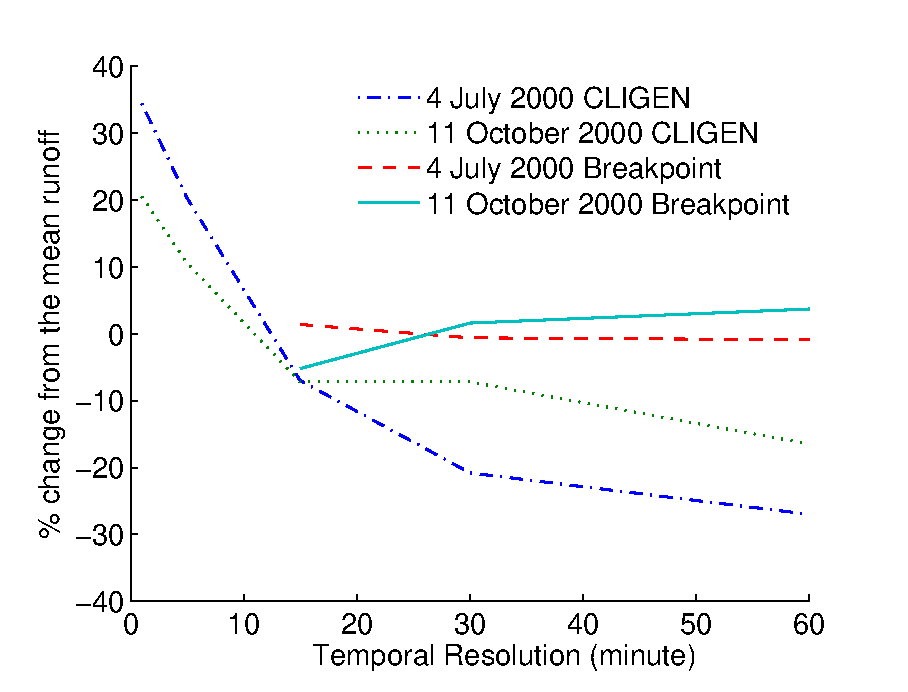
\includegraphics[width=0.70\textwidth]{./img/wepp_runoff_temp_scale}}
    \qquad
    \subfloat[][Changes in Soil
Loss]{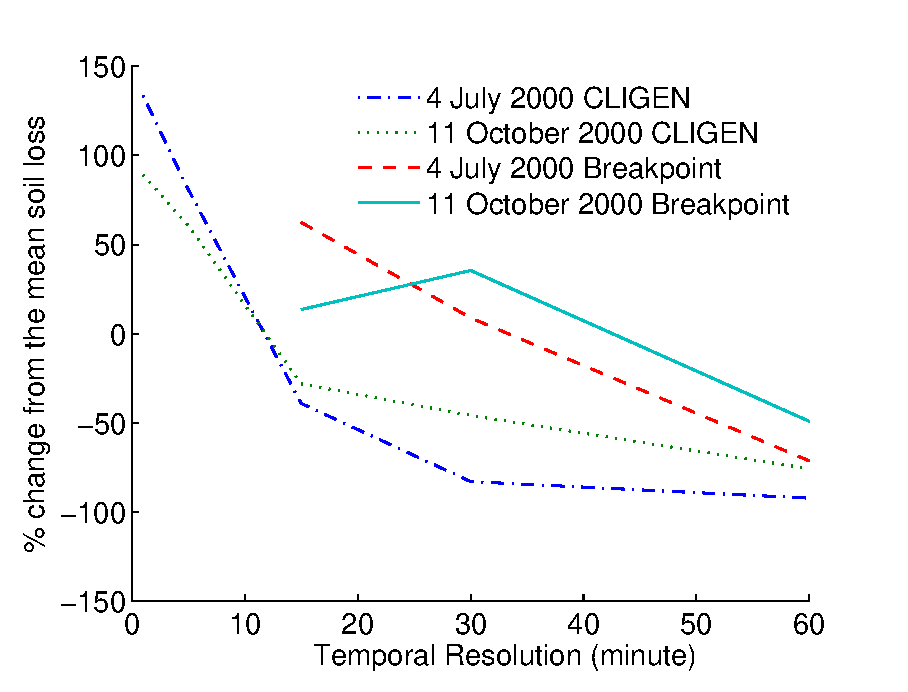
\includegraphics[width=0.70\textwidth]{./img/wepp_sloss_temp_scale}}
  \caption[WEPP runoff and soil loss changes]{The changes of WEPP simulated
runoff and soil loss from average runoff and soil loss. Note the scale of y-axis
in (b) Changes in Soil Loss.}
  \label{fig:wepp_roff_sloss_temp_scale}
\end{figure}

\begin{figure}[htbp]
  \centering
    \subfloat[][Changes in
Runoff]{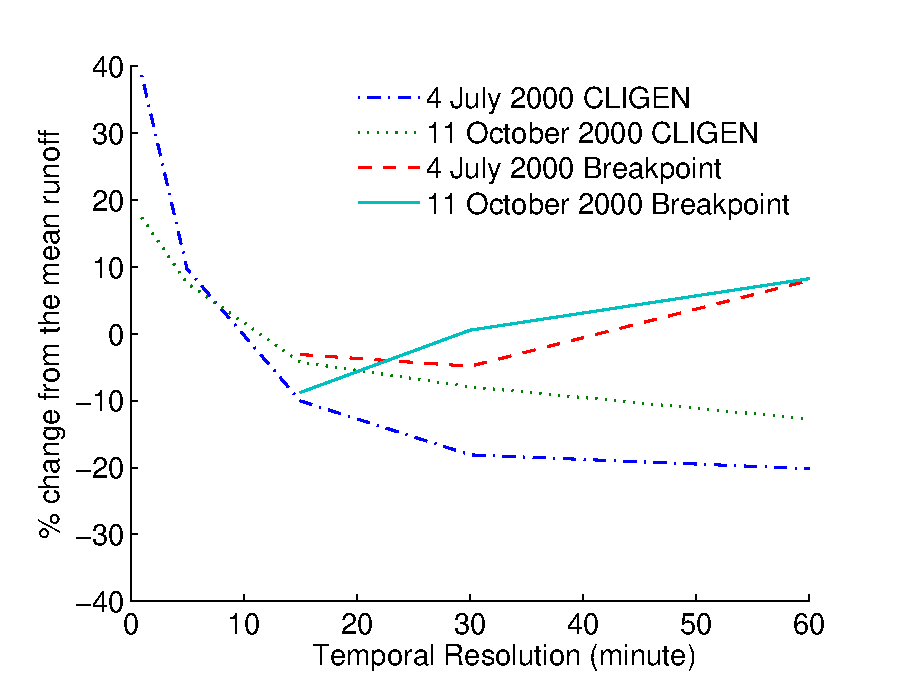
\includegraphics[width=0.70\textwidth]{./img/eurosem_roff_temp_scale}}
    \qquad
    \subfloat[][Changes in Soil
Loss]{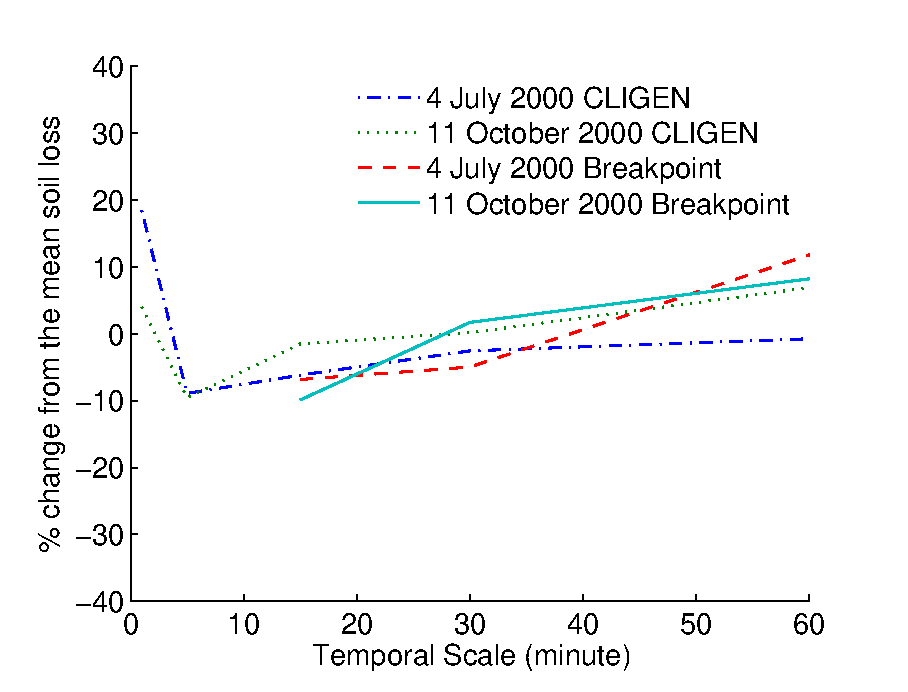
\includegraphics[width=0.70\textwidth]{./img/eurosem_sloss_temp_scale}}
  \caption{The changes of EUROSEM simulated runoff and soil loss from average
runoff and soil loss}
  \label{fig:eurosem_roff_sloss_temp_scale}
\end{figure}

Changes of temporal scales of CLIGEN rainfall data are inversely proportional
to WEPP simulated runoff and erosion rates. In comparison to 15-min data, CLIGEN
data with higher temporal resolution resulted in greater WEPP simulated runoff
and erosion rate than CLIGEN data with lower temporal resolution data.
When rainfall data are in breakpoint data forms, temporal data scales have a
varying effects on WEPP simulated runoff and erosion rate which do not show
clear relationships.

EUROSEM simulated runoff and erosion rate show rather different results from
WEPP simulations. Temporal data scales do have effects on runoff and erosion
rate simulation by EUROSEM as seen in Table
\ref{tab:DifferentTemporalScalesOfRainfallDataOnEUROSEMRunoffEstimation} and
\ref{tab:DifferentTemporalScalesOfRainfallDataOnEUROSEMSoilLoss} and Figure
\ref{fig:eurosem_roff_sloss_temp_scale}. However, the result is quite the
opposite from WEPP simulations. Breakpoint data with lower temporal resolution
resulted in moderate increases of both runoff and erosion rates by EUROSEM. In
contrast, CLIGEN data resulted in decreasing runoff and increasing soil loss
rates as temporal data scales increase. This result is rather odd because
decreasing runoff normally accompanied by decreasing soil erosion rate. Also,
5-min CLIGEN data is the only temporal scale that show decreased soil loss
compared to soil loss generated with 15-min CLIGEN data.

%Maybe because of detachment rate was more affected? Discuss this.

Between 1-min data and 60-min data, erosion rate was almost 8-30 times greater
when simulated with 1-min data than with 60-min data. This clearly is
problematic.

\section{Discussion}
\label{sec:TemporalScalesDiscussion}

%Uncertainty should be discussed
%cf \cite{jones1997-265,murphy2006-65,oberkampf2002-333,parsons2000-723}

Although WEPP documents states that 15-min data are to be used, the effect of
other temporal scales have been explored since 15-min data are not always
available for the erosion modelling studies. The results are compared in terms
of the rates of changes (\%) to highlight the relative effects of the changes
only.

Breakpoint data that are prepared for both July and October events with 1 and
5-min data could not be used for both models---WEPP and EUROSEM. This is because
WEPP limits the number of maximum breakpoint to 50 points per day according to
the model document \citep{flanagan1995-usda}. This means that, for a rainfall
event that last for a whole day, 30-min data is the highest resolution we can
use for WEPP simulations because there are 48 (24/0.5) intervals per day. This
prohibits the use of breakpoint data with temporal resolution higher than
30-min in theory. In practice, any temporal scale could be used as long as the
total number of breakpoints does not exceed 50 points. Testing with the most
up-to-date WEPP revealed that up to 100 breakpoints may be used without a
problem. However, when more than 100 breakpoints were used, WEPP does not
recognise the start and end of a rainfall event correctly, and re-aggregates the
rainfall with multiple starting times (i.e.\ 0 minute point). The maximum number
of breakpoints should be increased to at least 1440 points or more to enable
the use of 1-min data or higher temporal data. EUROSEM have the same limitation
which prevent from using more than 100 breakpoints. Also, total 1000 breakpoints
for simulations with multiple rainfall gauges. Clearly both models need to
increase their dimension of breakpoint data array to meet the need.

Rainfall parameters in the CLIGEN input file are originally calculated from
15-min (breakpoint) data. CLIGEN then uses this statistical information to
simulate continuous long-term daily rainfall data which has similar statistical
characteristics as the observed data in the form of four unique parameters
(rainfall amount, rainfall duration, normalised peak intensity and normalised
time to peak). These four parameters then were used by WEPP to disaggregate the
daily rainfall data into ten breakpoint data using a double exponential
function. This procedure is, however, highly inefficient in retaining original
rainfall intensity information, particularly for the event with a long duration
and low intensity which is similar to the event occured on 11 October 2000.
The rainfall information can be distorted or lost during these data
``conversion'' processes. An obvious reason why WEPP-CLIGEN use such
method seems to be because of the ease of use and data storage for long-term
records. This method---statistically summarising historical climate data and
maintaining it---is a very efficient way of storing a large amount of rainfall
data. One file (i.e.\ CLIGEN input file) per weather station requires much less
space than tipping-bucket data for, say, 10 to 20 years. This however does have
a couple of disadvantages:
\begin{enumerate*}
  \item The concept of CLIGEN data is only suitable for convective storms which
do not have many intermittent rainfall phases (no-rain periods) during rainfall.
\medskip
  \item For WEPP to disaggregate CLIGEN data realistically using a double
exponent function, each storm should have one distinctive high rainfall peak.
Such storms are not typical of many parts of the world, and may be seasonally
dependant.
\end{enumerate*}
It is, however, evident that CLIGEN data type make it easier to deal with vast
amounts of data. It also requires considerably less space to store such data.
Also, CLIGEN data are very good to use with WEPP as it is designed specifically
for such use.

The intensity information of rainfall data is heavily dependant on how they are
aggregated. When rainfall data such as tipping-bucket data are aggregated into
certain time steps, they are usually stored in a digitized data format. It means
the averaged rainfall intensity is dependant on the start time as well as
time-steps which is temporal scales. Time-steps and start time are important as
the rainfall intensity is averaged over the given time-steps and start point
when they are archived. This method, however, unintentionally discards rainfall
intensity information by averaging rainfall peaks over the given time step.

The effect of discarding rainfall intensity information has been clearly shown
when both events---i.e.\ rain storms on 4 July 2000 and 11 October 2000---are
aggregated into varying time steps. Distinctive high intensity peaks in 1-min
data (Figures \ref{fig:dr_storm-a} and \ref{fig:pl_storm-a}) was no more visible
as intensity was averaged out over the longer timestep data (See Figures
\ref{fig:dr_storm} and \ref{fig:pl_storm}).

Two effects can be noted when the temporal scale changes. One is the effect from
the lowering of the actual instantaneous peak intensity and average intensity of
the storms. The other is the effect from the location of the peak intensity
changes during each storm.

Lowering the average intensity means a reduced average power of erodibility of
the rain. Lowering the peak intensity means a reduced instantaneous peak power
of erodibility of the the rain. These changes may be a significant reason
for the underestimation of the runoff and soil loss. Shifting the location of
the peak rainfall intensity means changed rainfall shapes which may be closely
related to the timing of the runoff generations. All these changes will occur
together when the temporal scale of rainfall data is altered. Thus, what we
observed in this study may well be the end product from compound effects of
these two changes.

The instantaneous rainfall peak intensity may hold key answers to the processes
of dispersion of soil particles. It is known that intense rainfall may exceed
the soil infiltration rate faster, so that runoff may occur in a shorter time
after the start of the rainfall event compared with low intense rainfall.
\citet{wainwright2002-1271} carried out numerical experiments to test if
temporal variability of rainfall intensity during a storm can cause the decrease
in runoff coefficients with increasing slop length. They found that variability
of temporal scale in rainfall is a significant factor in controlling the
scale-dependency of runoff coefficients. Also, overland-flow models which use
mean rainfall intensities may notably under-predict the runoff.

High rainfall intensity is closely related to high rainfall kinetic energy,
which controls runoff generation and soil loss. Yet the way of archiving and
aggregating long term rainfall data may miss out important rainfall intensity
details as shown in this chapter. \citet{boardman1987-36} also pointed out that
short period high intensities probably important for soil erosion processes.

Short duration rainfall intensities are affected by a large uncertainty,
especially when they are produced during extreme convective rainfall events
\citep{garcia2001-675}. In the study by \citet{garcia2001-675}, 408 rainfall
events have been statistically analysed for the period 1925-1992 in Alicante
(Spain). Maximum intensities for durations ranging from 2 minutes up to 240
minutes were extracted from the series \citep{garcia2001-675}. Considerable
differences are found in the behaviour of the empirical functions for short
durations (t < 10 minutes) \citep{garcia2001-675}. The energy of individual
storms could only be predicted with limited accuracy because of natural
variations in rainfall characteristics \citep{vandijk2002-1}.

For future soil erosion studies, one needs to know about future rainfall
intensity. But without high resolution rainfall data, one may predict future
soil erosion with a large error as shown by this investigation.  Even with
15-min data it is possible to get as much as about 3 times less soil erosion
estimation compared to 1-min data. This may pose a problem when using large
scaled GCM or RCM rainfall data directly for soil erosion. It is relatively
difficult to predict rainfall intensity changes with good reliability even with
a climate model.

%It is known to be possible to simulate future climate with 30 or 20 min
%time steps, though this is for the whole grid, so that it is almost without
%meaningless information for erosion modelling. Still one may be able to run
%erosion model using direct outputs from GCMs with such high resolution, but
%?? what problems??.

High temporal resolution data are needed in order to describe the temporal
variation of rainfall intensities realistically. High temporal resolution data
captures in great detail rainfall intensity patterns including instant high
intensity peaks. However, such high resolution data are very rarely available.
As \citet{allott2002-73} pointed out, high-resolution data permit a more
detailed assessment of the storm structure and evolution of localised intense
storms, but storms are rarely monitored by sub-hourly recording rain gauges.
Even if storms are recorded by a sub-hour scale, often the records are
converted into hourly or daily for archiving. Thus, a little is ever known
about the storm structure and evolution. In many case, therefore, only hourly or
daily data are available. Even with hourly (or more generally daily data), the
actual rainfall intensity details can not be derived (Figure \ref{fig:pl_storm})
although this information about intensity may be particularly responsible for
the runoff and soil loss estimation using erosion models.

Therefore, it is clear that we need to use breakpoint rainfall data with high
resolution in order to keep the detail of rainfall intensity as well as
maintaining original characteristics of rainfall for erosion simulations.
However, high resolution breakpoint data will lead to erroneous simulation
results because of the model limitation (i.e.\ the maximum number of
breakpoints) as discussed previously. 1-min and 5-min data cannot be used.
Also, the temporal scale of hourly (60-min) data is too long to provide
detailed information of rainfall intensity. Now we have left with two choices:
15-min and 30-min data. Without a doubt, 15-min data were chosen because they
have greater details of rainfall intensity than 30-min data. Also, both WEPP
and EUROSEM can easily used 15-min breakpoint data. It is however important to
note that erosion models should be able to take high resolution data such as
1-min breakpoint data and work reasonably well for testing and estimations of
erosion.

\section{Conclusion}
\label{sec:TemporalScalesConclusion}

Higher resolution dose not always give a better simulation result.
Equally low resolution data dose not mean worse simulation results. It can be a
problem however when we do not have high resolution data but only low resolution
(60-min) data because we will never know what the intensity was like during
those 60-min. Also, with no knowledge of the intensity information, simulation
results can be anywhere between 8 to 30 times different from ``original
results''. This figure is so great that it might mean from almost no erosion to
disastrous events.

%What temporal scaled rainfall data should I suppose to use? and why?
%What can we expect to happen if we use other temporal data?
In this chapter, the following was found:
\begin{itemize}
  \item Temporal scales of rainfall data are closely related to the results of
runoff and soil loss modelling
  \item High resolution CLIGEN data generally yield more runoff and soil loss
  \item Temporal scales of rainfall data affect estimations of soil loss more
than runoff
  \item Effects of the temporal data scale is greater for the summer rainfall
event (event on 4 July 2000)
  \item For the purpose of soil erosion simulation, 15-min breakpoint rainfall
data are chosen
  \item It may be suggested to use breakpoint data for the further simulations
in this research
\end{itemize}

It is also recognised that different ways of expressing rainfall intensity have
the tenancy of desirability for erosion modelling. This is summarised in Table
\ref{tab:DesirabilityOfDifferentWaysOfExpressingRainfallIntensity}.

\begin{table}[htbp]
  \small
  \centering
      \caption{Desirability of different ways of expressing rainfall intensity}
  \label{tab:DesirabilityOfDifferentWaysOfExpressingRainfallIntensity}
    \begin{tabular}{ccl}
    \toprule
    Similarity to Reality & Desirability & Method of Rainfall Data
Representation\\
    \midrule
    Dissimilar & Most & Amount, Duration, Time-to-Peak \& Peak Intensity\\
    $\uparrow$ & $\uparrow$ &  Breakpoint Data without `no rainfall periods'\\
    $\downarrow$ & $\downarrow$ &  Breakpoint Data with `no rainfall periods'\\
    Similar & Least & Tipping Bucket Data\\
    \bottomrule
    \end{tabular}
\end{table}

Even though breakpoint data hold more information and are closer to real
rainfall than CLIGEN data, it still has some problems. The temporal scale of
breakpoint data limits their closeness to real rainfall since rainfall intensity
is averaged between starting and ending time of breakpoints.

This chapter is followed by a further research question: `\textit{What is the
consequence of removing the no-rain periods within a storm in order to estimate
CLIGEN data?}'.
%This question can be answered by the continuous and discontinuous storm test in
%Chapter \ref{sec:EFFECTSOFCONTINOUSANDDISCONTINUSSTORM}.
The suggested test raises an issue about the no-rain periods that are removed
during CLIGEN data preparation which, in turn, may lead to a loss of rainfall
intensity information. More worryingly distorting rainfall intensity information
and feeding this wrong information into soil erosion models could occur. Thus,
only one storm that has few recognizable intermittent no-rain periods within the
storm duration is subjectively selected and tested in the next chapter.

%******put B2B test here (intensity burst test)


%\nolinenumbers

%%%%%%%%%%%%%%%%%%%%%%%%%%%%%%%%%%%%%%%%%%%%%%%%%%%%%%%%%%%%%%%%%%%%%%%%%%%%
%\section{Discussion on CLIGEN versus Breakpoint Data}
%\label{sec:tpipbpIntroduction}
%
%When rainfall data are used for erosion modelling, two data types are
%available---CLIGEN and breakpoint data. In this section, these two rainfall
%data types are compared in terms of runoff and soil loss generations using
%WEPP and EUROSEM.
%
%This section aims to determine which rainfall data input method is more
%desirable for the subsequent investigations of the effect of rainfall
%intensity on soil erosion.
%
%The storm observed on 4 July 2000 is a typical summer rainfall event in the
%UK. It has a relatively short duration with a rapid rainfall intensity
%change during the storm period. The storm which fell on 11 October 2000
%with a longer duration can typically be observed in the British autumn
%periods. It sometimes lasts over few days with a gradual rainfall intensity
%change, often followed by severe floods.
%
%Original peak intensity of the storm is unchanged. Only duration is changed
%because of removal of no-rain periods from the total storm duration.
%
%This may be a problem as it clearly does not use the same data directly.
%However, as WEPP also uses the same 10 breakpoint data disaggregated from
%CLIGEN data, there should not be any differences in the values used for
%calculating runoff and soil loss. Moreover, this test is to find out what
%rainfall intensity information we might miss out by using one data form
%instead of another, and the consequence of using such data. This means that
%the efficiency of each data form is not the main interest here although it
%might be related to the actual outcomes of this test.
%
%As there is no observed runoff and soil loss data, it may be difficult to
%prove which data type gives better (or realistic) erosion results. Thus,
%each data type is compared in terms of characteristic differences. %pros
%and cons, closeness to real rainfall patterns, retaining intensity
%information can be discussed here.
%Does it have no artefacts in simulating erosion? (This is as mentioned
%difficult to find because of no measurement) Does it really matter for
%erosion estimation? rainfall duration? Is the differences in the result
%obvious? Did the result really show clearly breakpoint data type is
%superior and preferred type over the CLIGEN data type? Is the result true
%for both storm? (very unlikely!)


%\subsection{Conclusion}
%\label{sec:tpipbpConclusion}

%Which type of the data provide more realistic information on rainfall
%intensity?

%\section{Suggestions for Further Investigations}
%\label{sec:FurtherInvestigationSuggestion}
%%%%%%%%%%%%%%
%You need to think about the order of chapters in the next part.
%temporal scale, intensity patterns, and gaps

%Use Tony's work and rillgrow in intensity pattern. this then give you the
%reason for using rillgrow result as reference in gap test.
%
%Ask all the questions that are going to be addressed in the next part.
%%%%%%%%%%%%%%
%This chapter is followed by a number of further research questions.

%One is that, if we choose to use breakpoint data over CLIGEN data, what is
%the appropriate data scale to use? Any sub-daily data are going to be good
%enough? Moreover, CLIGEN rainfall parameters (precipitation amount  (mm),
%$R$, storm duration (hour), $D$, time to peak as a fraction of the storm
%duration, $t_p$, and the ratio of peak  intensity over average intensity,
%$i_p$) are calculated originally from 15-min rainfall data. This, however,
%overlooks the variations of rainfall intensity within 15 minutes.
%Therefore, it is suggested to test effects of different temporal scale of
%data on soil erosion.

%The second question is `What are the consequence of removing the no-rain
%periods within a storm in order to estimate CLIGEN data?'. Is this going to
%be ok to just ignore these intermittent rainfall pattern and consider them
%as a continuous rainfall? These questions can be answered by continuous and
%discontinuous storm test.

%This continuous and discontinuous storm test may seem very similar to the
%previous test discussed just now. But, it is not!

%Let's be clear about this. comparison done between BP and CLIGEN data is to
%find which type of data representation is better than the other for erosion
%simulation. So, two different types of storms are chosen for the test.

%The suggested test (second one) raises an issue about the no-rain periods
%that is removed during data preparation, which in turn, may lead to a loss
%of rainfall intensity information. more worryingly distorting rainfall
%intensity information and feed this wrong data into soil erosion models.
%So, only one storm that has few recognizable intermittent gaps within the
%storm duration is subjectively selected and tested.
